\documentclass{beamer}
\usepackage[english,russian]{babel}
\usepackage[utf8]{inputenc}
\usepackage{listings}
\usepackage{color}
\usepackage{xcolor}
\usepackage{ucs}
\lstset{inputencoding=utf8x, extendedchars=\true, captionpos=b, tabsize=3, keywordstyle=\color{blue},commentstyle=\color{green}, stringstyle=\color{red}, showstringspaces=false, basicstyle=\footnotesize,emph={label}, texcl}
%\lstset{texcl}
%\lstset{extendedchars=\true}
\lstset{
literate={а}{{\selectfont\char224}}1
{б}{{\selectfont\char225}}1
{в}{{\selectfont\char226}}1
{г}{{\selectfont\char227}}1
{д}{{\selectfont\char228}}1
{е}{{\selectfont\char229}}1
{ё}{{\"e}}1
{ж}{{\selectfont\char230}}1
{з}{{\selectfont\char231}}1
{и}{{\selectfont\char232}}1
{й}{{\selectfont\char233}}1
{к}{{\selectfont\char234}}1
{л}{{\selectfont\char235}}1
{м}{{\selectfont\char236}}1
{н}{{\selectfont\char237}}1
{о}{{\selectfont\char238}}1
{п}{{\selectfont\char239}}1
{р}{{\selectfont\char240}}1
{с}{{\selectfont\char241}}1
{т}{{\selectfont\char242}}1
{у}{{\selectfont\char243}}1
{ф}{{\selectfont\char244}}1
{х}{{\selectfont\char245}}1
{ц}{{\selectfont\char246}}1
{ч}{{\selectfont\char247}}1
{ш}{{\selectfont\char248}}1
{щ}{{\selectfont\char249}}1
{ъ}{{\selectfont\char250}}1
{ы}{{\selectfont\char251}}1
{ь}{{\selectfont\char252}}1
{э}{{\selectfont\char253}}1
{ю}{{\selectfont\char254}}1
{я}{{\selectfont\char255}}1
{А}{{\selectfont\char192}}1
{Б}{{\selectfont\char193}}1
{В}{{\selectfont\char194}}1
{Г}{{\selectfont\char195}}1
{Д}{{\selectfont\char196}}1
{Е}{{\selectfont\char197}}1
{Ё}{{\"E}}1
{Ж}{{\selectfont\char198}}1
{З}{{\selectfont\char199}}1
{И}{{\selectfont\char200}}1
{Й}{{\selectfont\char201}}1
{К}{{\selectfont\char202}}1
{Л}{{\selectfont\char203}}1
{М}{{\selectfont\char204}}1
{Н}{{\selectfont\char205}}1
{О}{{\selectfont\char206}}1
{П}{{\selectfont\char207}}1
{Р}{{\selectfont\char208}}1
{С}{{\selectfont\char209}}1
{Т}{{\selectfont\char210}}1
{У}{{\selectfont\char211}}1
{Ф}{{\selectfont\char212}}1
{Х}{{\selectfont\char213}}1
{Ц}{{\selectfont\char214}}1
{Ч}{{\selectfont\char215}}1
{Ш}{{\selectfont\char216}}1
{Щ}{{\selectfont\char217}}1
{Ъ}{{\selectfont\char218}}1
{Ы}{{\selectfont\char219}}1
{Ь}{{\selectfont\char220}}1
{Э}{{\selectfont\char221}}1
{Ю}{{\selectfont\char222}}1
{Я}{{\selectfont\char223}}1
}
% Стиль презентации
\usetheme{Madrid}
\begin{document}
\title{Квантовые языки программирования}  
\author[Донцов А.]{Донцов Александр\inst{1}, 571 гр.}

\institute[АлтГУ]
{	\inst{1}%
ГОУ ВПО <<Алтайский государственный университет>>\\
Кафедра радиофизики и теоретической физики
}

\date{
   Барнаул\\
    2012г.
}
\begin{frame}
\begin{block}{}
\begin{center}
ФГБОУ ВПО <<Алтайский государственный университет>>\\
Физико-технический факультет\\
Кафедра радиофизики и теоретической физики
\end{center}
\end{block}
  \begin{columns}
    \column{.9\textwidth}
      \begin{block}{}
	\begin{flushleft}
	  {{\Large \bf Физическая реализация квантовых вычислений на основе квантовых точек\\}}
	\end{flushleft}
      \end{block}
    \column{.1\textwidth}
  \end{columns}
\begin{center}
\textbf{Донцов Александр Андреевич}
\end{center}
  \begin{columns}
    \column{.8\textwidth}
      \begin{flushright}
      \end{flushright}
    \column{.2\textwidth}
  \end{columns}

  \begin{columns}
    \column{.1\textwidth}
    \column{.9\textwidth}
      \begin{flushright}
	Научный руководитель: к.ф.-м.н. Н.\,В. Волков\\
      \end{flushright}
  \end{columns}
\end{frame}
\begin{frame}
 \frametitle{Актуальность}
В настоящее время сделана большая работа в области построения квантовых вычислительных машин, разработана большая теоретическая база. Хотя до сих пор полноценный квантовый компьютер не был построен, но уже сейчас реализованы некоторые прототипы квантового компьютера. Для реализации квантовых алгоритмов нужно выполнить следующие условия:
  
\begin{itemize}
  \item адекватно представлять квантовую информацию; 
 
  \item выполнять универсальный набор квантовых унитарных преобразований;

  \item приготавливать начальное состояние;
  
  \item измерять конечный результат.
\end{itemize}

\end{frame}
\begin{frame}
\frametitle{Квантовая точка, квантовый гармонический осциллятор}
\begin{block}{Квантовая точка, квантовый гармонический осциллятор}
Квантовая точка --- это фрагмент проводника или полупроводника, содержащий в себе электрон или электроны, ограниченные со всех сторон каким-либо потенциальным барьером, в качестве барьера довольно часть применяют примеси каких-либо других веществ. Потенциал, создаваемый в квантовой точке,
ограничивает движение носителей заряда во всех трёх пространственных измерениях. Характерные размеры квантовой точки от 10 нм до 100 нм.
\end{block}
\end{frame}
\begin{frame}
\frametitle{Вычисления}
\begin{eqnarray}
|00\rangle_{L} \longleftrightarrow |0\rangle,   \\
|01\rangle_{L} \longleftrightarrow |1\rangle,\\
|10\rangle_{L} \longleftrightarrow \frac{|0\rangle + |1\rangle}{\sqrt{2}} \label{plus-position},\\
|10\rangle_{L} \longleftrightarrow \frac{|0\rangle - |1\rangle}{\sqrt{2}} \label{minus-position}.
\end{eqnarray}
\begin{figure}[h]
\centering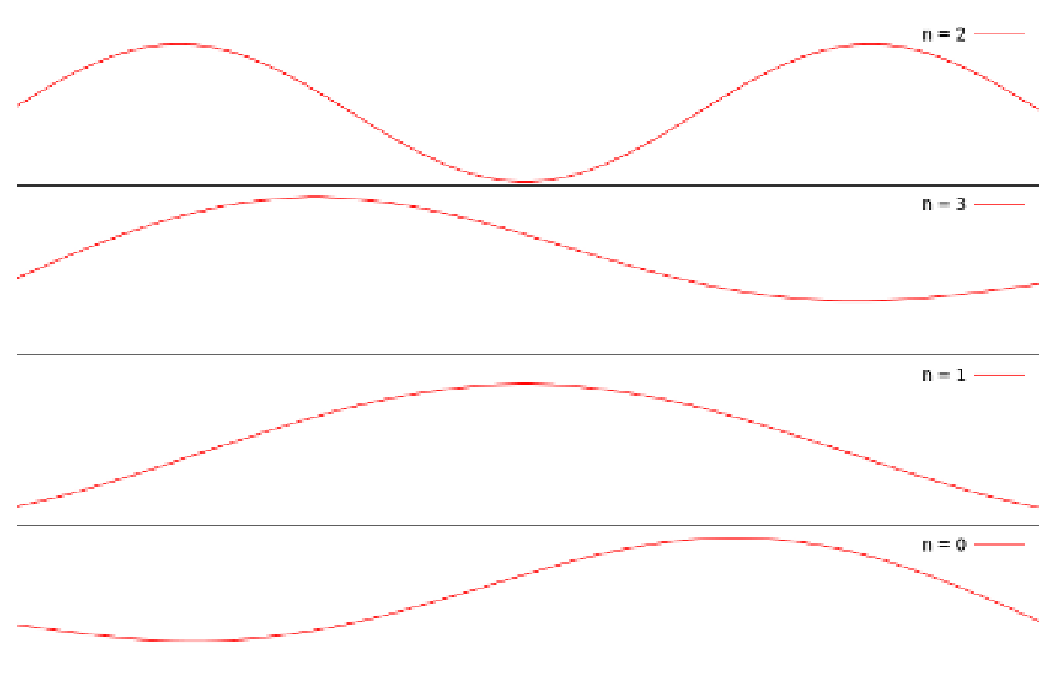
\includegraphics[width=.50\textwidth]{images/function.eps}
\caption{Собственные функции гармонического осциллятора}\label{ris:kk1}
\end{figure}

\end{frame}
\begin{frame}
\begin{figure}[h]
\begin{minipage}[h]{0.49\linewidth}
\center{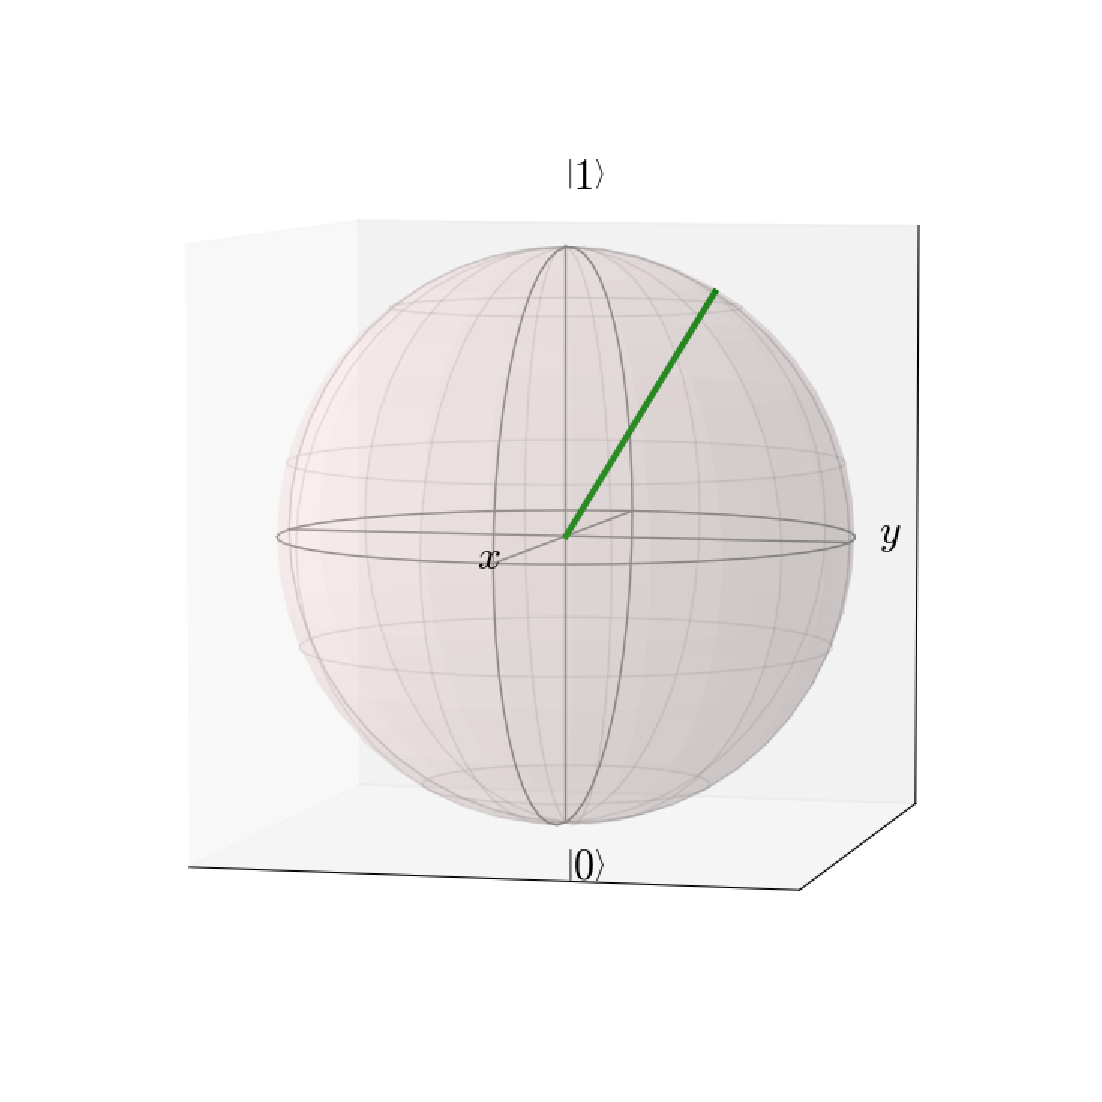
\includegraphics[width=.80\textwidth]{images/bloh1.eps} \\ а)}
\end{minipage}
\hfill
\begin{minipage}[h]{0.49\linewidth}
\center{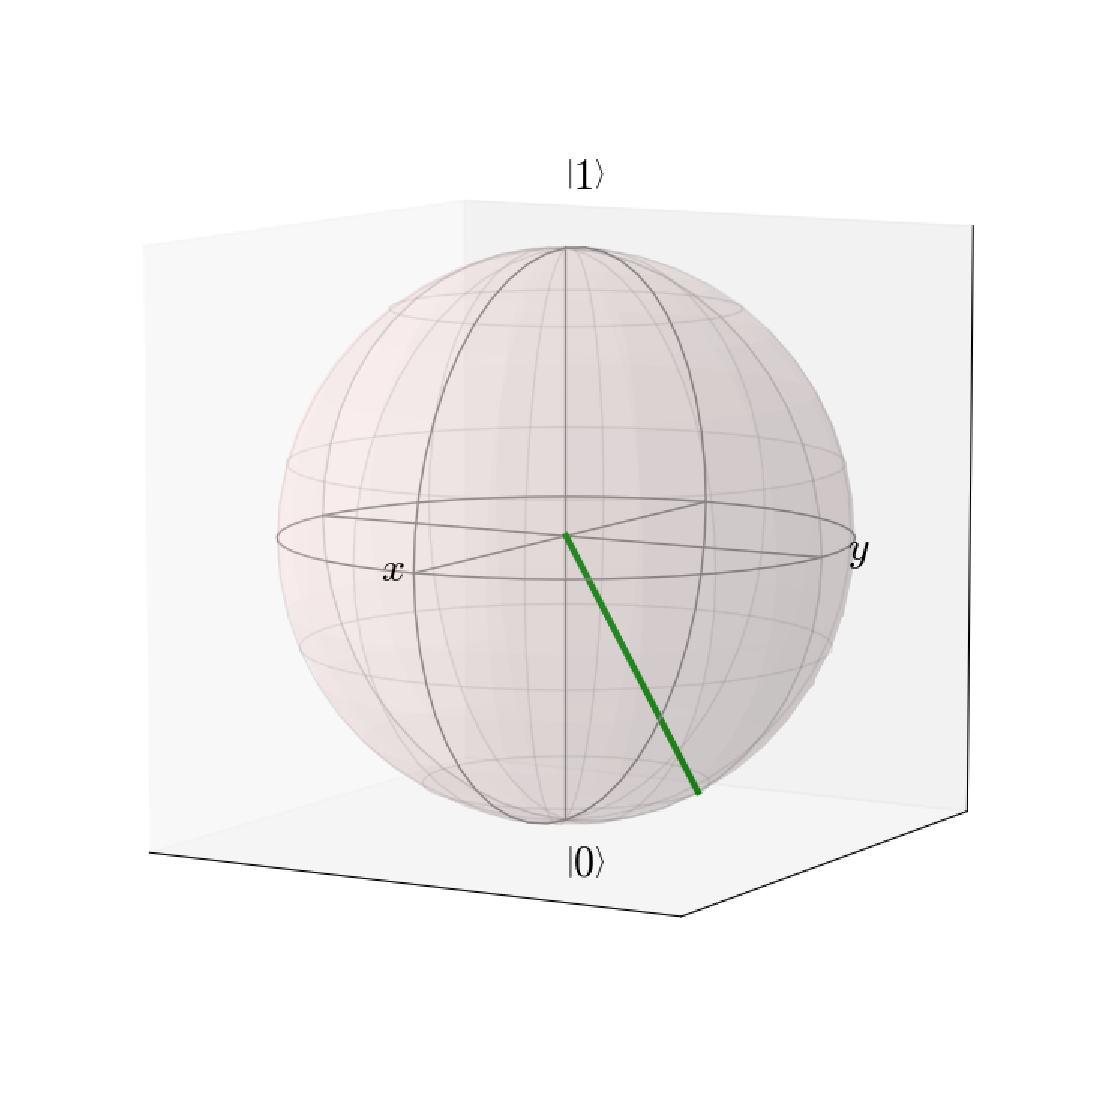
\includegraphics[width=.80\textwidth]{images/bloh2.eps} \\ б)}
\end{minipage}
\caption{Состояния (\ref{plus-position}) и (\ref{minus-position}) изображеные на сфере Блоха}
\label{ris:image1}
\end{figure}
\end{frame}
\begin{frame}
 \frametitle{Результаты}
В ходе данной работы были получены следующие результаты:
\begin{itemize}
  \item Получено решение задачи вычисления спектра и собственных функций квантовой точки.
  \item Показано, что данная задача может быть переформулирована, как задача проведения квантовых вычислений, в которой в качестве кубита выступает электрон, помещённый в квантовую точку, а в качестве унитарного квантового оператора выступает магнитное поле.
 \end{itemize}
\end{frame}
\end{document}